\section{ HÀM SỐ BẬC HAI}
\subsection{TÓM TẮT LÝ THUYẾT}

\subsubsection{Hàm số bậc hai $y=ax^2+bx+c$, với $a \ne 0$.}
	\begin{itemize}
			\item[\ding{172}] Tập xác định $\mathbb{R}$.
			\item [\ding{173}] Tọa độ đỉnh $S\left(-\dfrac{b}{2a};-\dfrac{\Delta}{4a} \right)$. \textit{Để xác định nhanh tọa độ đỉnh, ta chỉ cần xác định hoành độ $x_0$. Sau đó thay $x_0$ vào hàm số, ta tính $y_0$}.
			\item [\ding{174}] Sự biến thiên của hàm số bậc hai:
			\begin{center}
				\begin{minipage}[b]{7cm}
					\begin{khung4}{$a>0$}
						
\begin{tikzpicture}
							\tkzTabInit[lgt=1,espcl=2]
							{$x$/1,$y$/2}
							{$-\infty$,$-\dfrac{b}{2a}$,$+\infty$}
							\tkzTabVar{+/$+\infty$,-/$-\dfrac{\Delta}{4a}$,+/$+\infty$}
						\end{tikzpicture}
						\begin{itemize}
							\item $a>0$ thì bề lõm quay lên.
							\item Hàm số nghịch biến trên $\left(-\infty;-\frac{b}{2a} \right)$; đồng biến trên $\left(-\frac{b}{2a};+\infty \right)$.
						\end{itemize}
					\end{khung4}
				\end{minipage}\hspace{1cm}
				\begin{minipage}[b]{7cm}
					\begin{khung4}{$a<0$}
						
\begin{tikzpicture}
							\tkzTabInit[lgt=1,espcl=2]
							{$x$/1,$y$/2}
							{$-\infty$,$-\dfrac{b}{2a}$,$+\infty$}
							\tkzTabVar{-/$-\infty$,+/$-\dfrac{\Delta}{4a}$,-/$-\infty$}
						\end{tikzpicture}
						\begin{itemize}
							\item $a<0$ thì bề lõm quay xuống.
							\item Hàm số đồng biến trên $\left(-\infty;-\frac{b}{2a} \right)$; nghịch biến trên $\left(-\frac{b}{2a};+\infty \right)$.
						\end{itemize}
					\end{khung4}
				\end{minipage}
			\end{center}
	\end{itemize}

\subsubsection{Đồ thị hàm số bậc hai $y=ax^2+bx+c$, với $a \ne 0$.}

		\begin{itemize}
			\item [\ding{172}] Trong mặt phẳng $Oxy$, đồ thị là một parabol:\\
			\hspace*{1cm}
			\begin{tikzpicture}[smooth,samples=300,scale=0.6,>=stealth]
			\draw[->] (-0.8,0)--(4.5,0) node[below]{$x$};
			\draw[->] (0,-1.5)--(0,2.5) node[right]{$y$};
			\draw (0,0) node[above left]{$O$};
			\draw[thick, magenta,domain=0.3:3.7] plot(\x,{(\x)^2-4*(\x)+3});
			\draw[fill=blue] (2,-1) circle(1.5pt) (2,0) circle(1pt) (0,-1) circle(1pt);
			\draw[dashed] (2,-1.5)--(2,2.5) (2,-1)--(0,-1)node[left]{\footnotesize$-\dfrac{\Delta}{4a}$};
			\node[right] at (2,2.4) {\footnotesize $x=-\tfrac{b}{2a}$};
			\node[right] at (0.5,-2) {\fbox{\footnotesize$a>0$}};
			\end{tikzpicture}
			\hspace*{4cm}
			\begin{tikzpicture}[smooth,samples=300,scale=0.6,>=stealth]
			\draw[->] (-0.8,0)--(4.5,0) node[below]{$x$};
			\draw[->] (0,-1.5)--(0,2.5) node[right]{$y$};
			\draw (0,0) node[above left]{$O$};
			\draw[thick, magenta,domain=0.2:3.8] plot(\x,{-(\x)^2+4*(\x)-2});
			\draw[fill=blue] (2,2) circle(1.5pt) (2,0) circle(1pt) (0,2) circle(1pt);
			\draw[dashed] (2,-1.4)--(2,2.5) (2,2)--(0,2)node[left]{\footnotesize$-\dfrac{\Delta}{4a}$};
			\node[right] at (2,-1.5) {\footnotesize $x=-\tfrac{b}{2a}$};
			\node[right] at (0.5,-2) {\fbox{\footnotesize$a<0$}};
			\end{tikzpicture}
			\item [\ding{173}] Trục đối xứng: $x=-\dfrac{b}{2a}$ (\textit{xem đồ thị}).
			\item [\ding{174}] Cắt trục tung tại điểm có tung độ bằng $c$, tức là đồ thị luôn qua điểm $(0;c)$.
			\item [\ding{175}] Giá trị lớn nhất (max), giá trị nhỏ nhất (min)
			\begin{itemize}
				\item Khi $a>0$, hàm số đạt \textbf{giá trị nhỏ nhất} $y_{\min} =-\dfrac{\Delta}{4a}$ khi $x=-\dfrac{b}{2a}$ (tại đỉnh).
				\item Khi $a<0$, hàm số đạt \textbf{giá trị lớn nhất} $y_{\max} =-\dfrac{\Delta}{4a}$ khi $x=-\dfrac{b}{2a}$ (tại đỉnh).
			\end{itemize}
		\end{itemize}
